\documentclass[final]{beamer}
\setbeamertemplate{navigation symbols}{}
\usepackage[size=a0,scale=1.55]{beamerposter}

\usetheme{Berlin}

\usepackage{graphicx}

\usepackage{booktabs}

\usepackage{cite}

\usepackage{hyperref}

\usepackage{pgfplotstable} 
\usepackage{pgfplots}
\pgfplotsset{compat=1.17}

\usepackage{caption}

\settowidth{\leftmargini}{\usebeamertemplate{itemize item}}
\addtolength{\leftmargini}{2\labelsep}

\usepackage[utf8]{inputenc}
\usepackage[T1]{fontenc}
\usepackage[scale=0.8]{newpxtext} 

\usepackage{tikz}
\usetikzlibrary{shapes, arrows.meta, positioning}

\usepackage{setspace}
\setstretch{1.05}

\title{Innovating for Impact \\ Designing Solutions to Economic and Social Challenges}
\author{Huixiaqing Liu - fhnp96}
\institute{Topic: An application of one or more innovation methods to an economic / social challenge that may be in the current media}
\date{\today}


\begin{document}
\begin{frame}{}
	\vspace{-1.4cm}


	\begin{columns}[t]

		% Column 1		
		\begin{column}{.3\linewidth}

			\begin{block}{Design Thinking}
				Design Thinking is a user-centric approach to innovation that emphasizes empathy, problem definition, ideation, prototyping and testing.

				\begin{enumerate}
					\item \textbf{Empathize:} Understand the user's needs, desires and challenges
					\item \textbf{Define:} Clearly articulate the problem statement based on user insights
					\item \textbf{Ideate:} Brainstorm a wide range of creative ideas to address the problem
					\item \textbf{Prototype:} Build tangible representations of selected ideas for experimentation
					\item \textbf{Test:} Engage users to gather feedback and refine the prototypes iteratively
				\end{enumerate}
				\vspace{0.67cm}
				\begin{figure}
					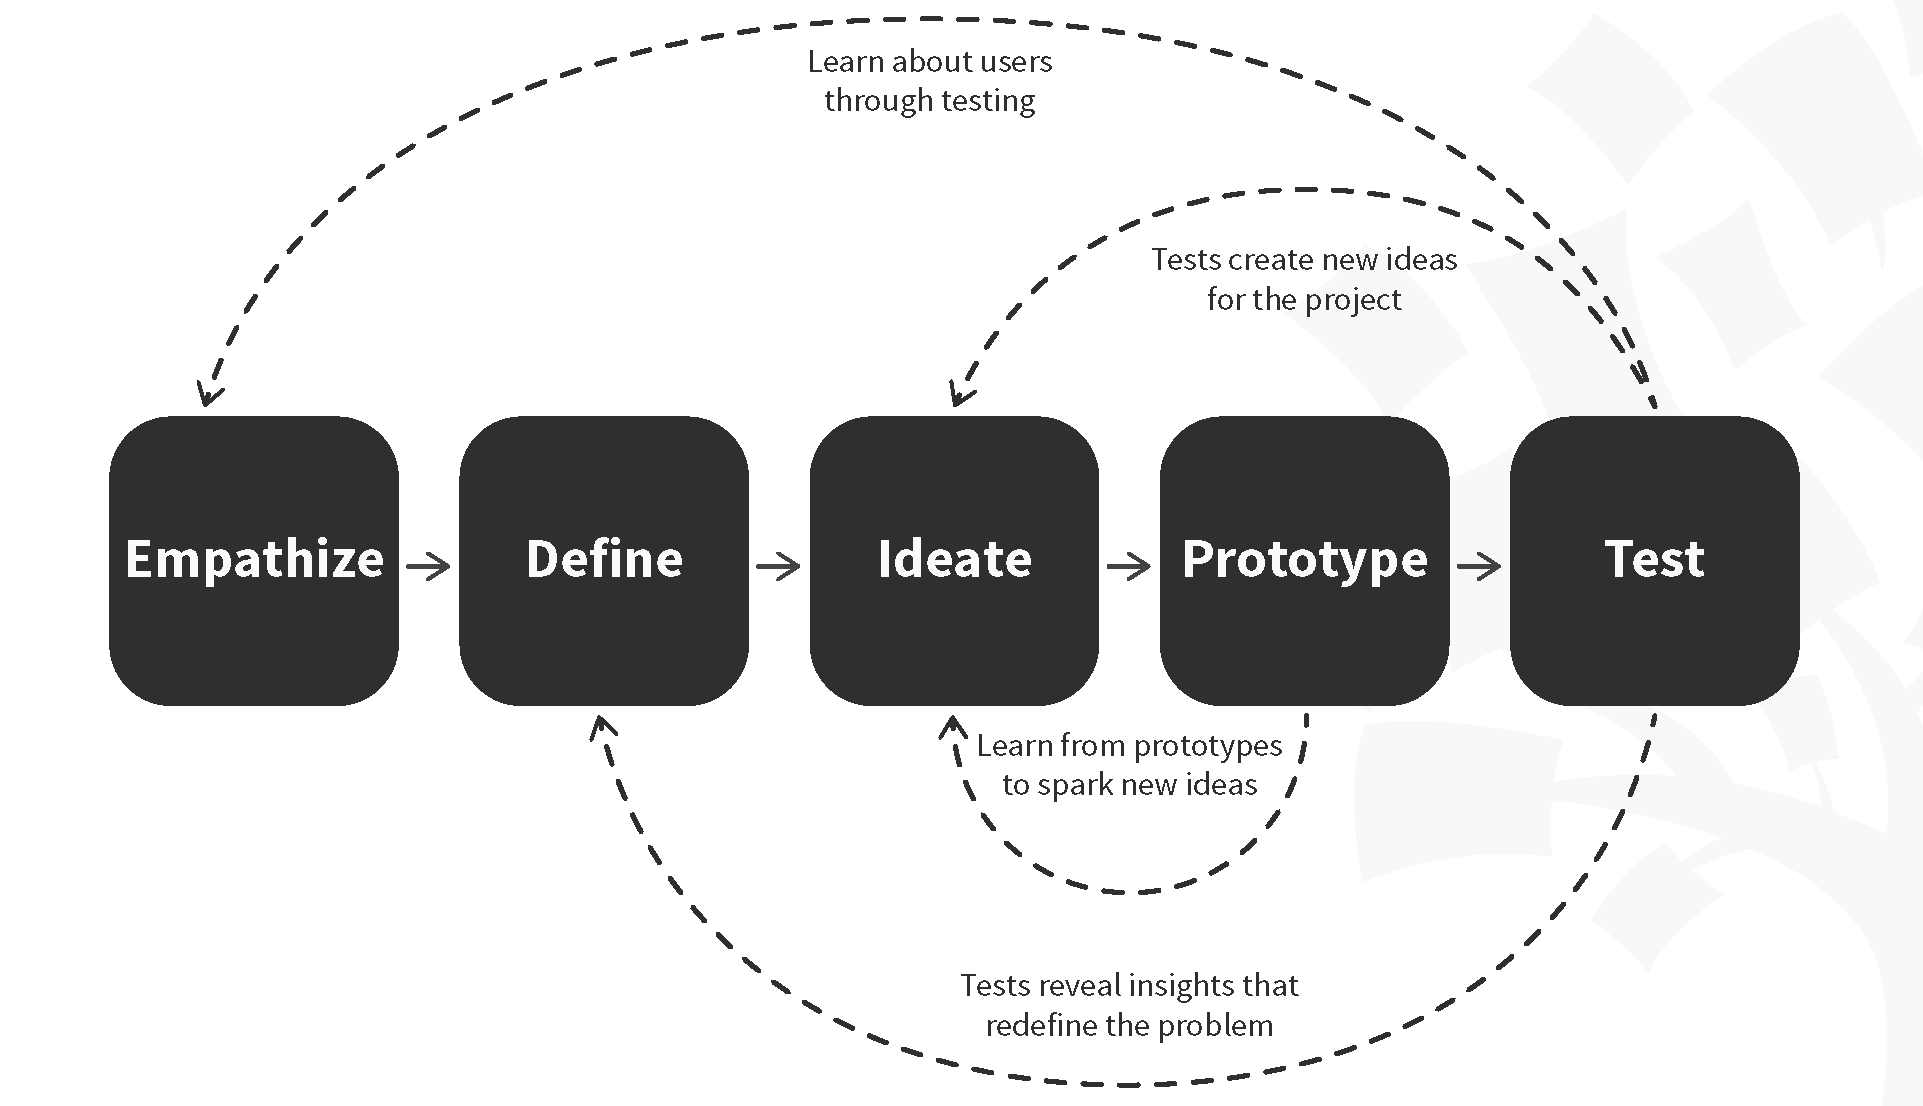
\includegraphics[width=\linewidth]{./images/design_thinking_process.png}
					\caption{The Five Stages of Design Thinking Process}
				\end{figure}

			\end{block}
			\vspace{1cm}
			\begin{block}{Key Benefits of Design Thinking}
				\begin{itemize}
					\item Fosters empathy and human-centric design
					\item Encourages exploration of a wide solution space
					\item Enables rapid learning through iterative prototyping and testing
					\item Suitable for tackling ill-defined, complex, people-oriented challenges
				\end{itemize}
			\end{block}
			\vspace{1cm}
			\begin{block}{Application to Economic Challenges}
				The COVID-19 pandemic has disrupted global supply chains. Applying the Design Thinking approach will help this issue in the following steps.
				\begin{enumerate}
					\item \textbf{Empathize} with customers struggling with product shortages and delays
					\item \textbf{Define} the problem as building resilient and agile supply networks
					\item \textbf{Ideate} strategies like diversifying suppliers, localizing production, and digitizing logistics
					\item \textbf{Prototype} new supply chain configurations and information systems
					\item \textbf{Test} and adapt the solutions based on performance during disruptions
				\end{enumerate}
			\end{block}

		\end{column}

		% Column 2
		\begin{column}{.35\linewidth}
			\vspace{-0.82cm}
			\begin{block}{}
				\centering
				\Large \textbf{\inserttitle}\\

				\vspace{0.8cm}

				\normalsize \insertauthor\\

				\vspace{0.85cm}
				
				\tiny \textit{\insertinstitute}
				
				\vspace{1cm}

			\end{block}
			\vspace{1cm}

			\begin{block}{Introduction}
				Innovation methods are powerful tools for:
				\begin{itemize}
					\item Generating novel ideas to solve complex problems
					\item Driving user-centric design and empathy
					\item Systematically analyzing and resolving technical contradictions
					\item Accelerating progress on critical economic and social challenges
				\end{itemize}
				This poster explores the application of \textbf{Design Thinking} and \textbf{TRIZ} to real-world issues.
			\end{block}
			\vspace{1cm}
			\begin{block}{TRIZ}
				TRIZ (Theory of Inventive Problem Solving) is a systematic approach that uses 40 inventive principles and contradiction matrices to resolve technical conflicts. It follows four key steps:
				\begin{enumerate}
					\item Identify the problem and its contradictions
					\item Find previously well-solved problems using contradiction matrices
					\item Look for analogous solutions and adapt to current problem
					\item Evaluate and implement the most promising solutions
				\end{enumerate}
				\vspace{1cm}

				\begin{figure}
					\centering
					\begin{minipage}{0.63\linewidth}
						\centering
						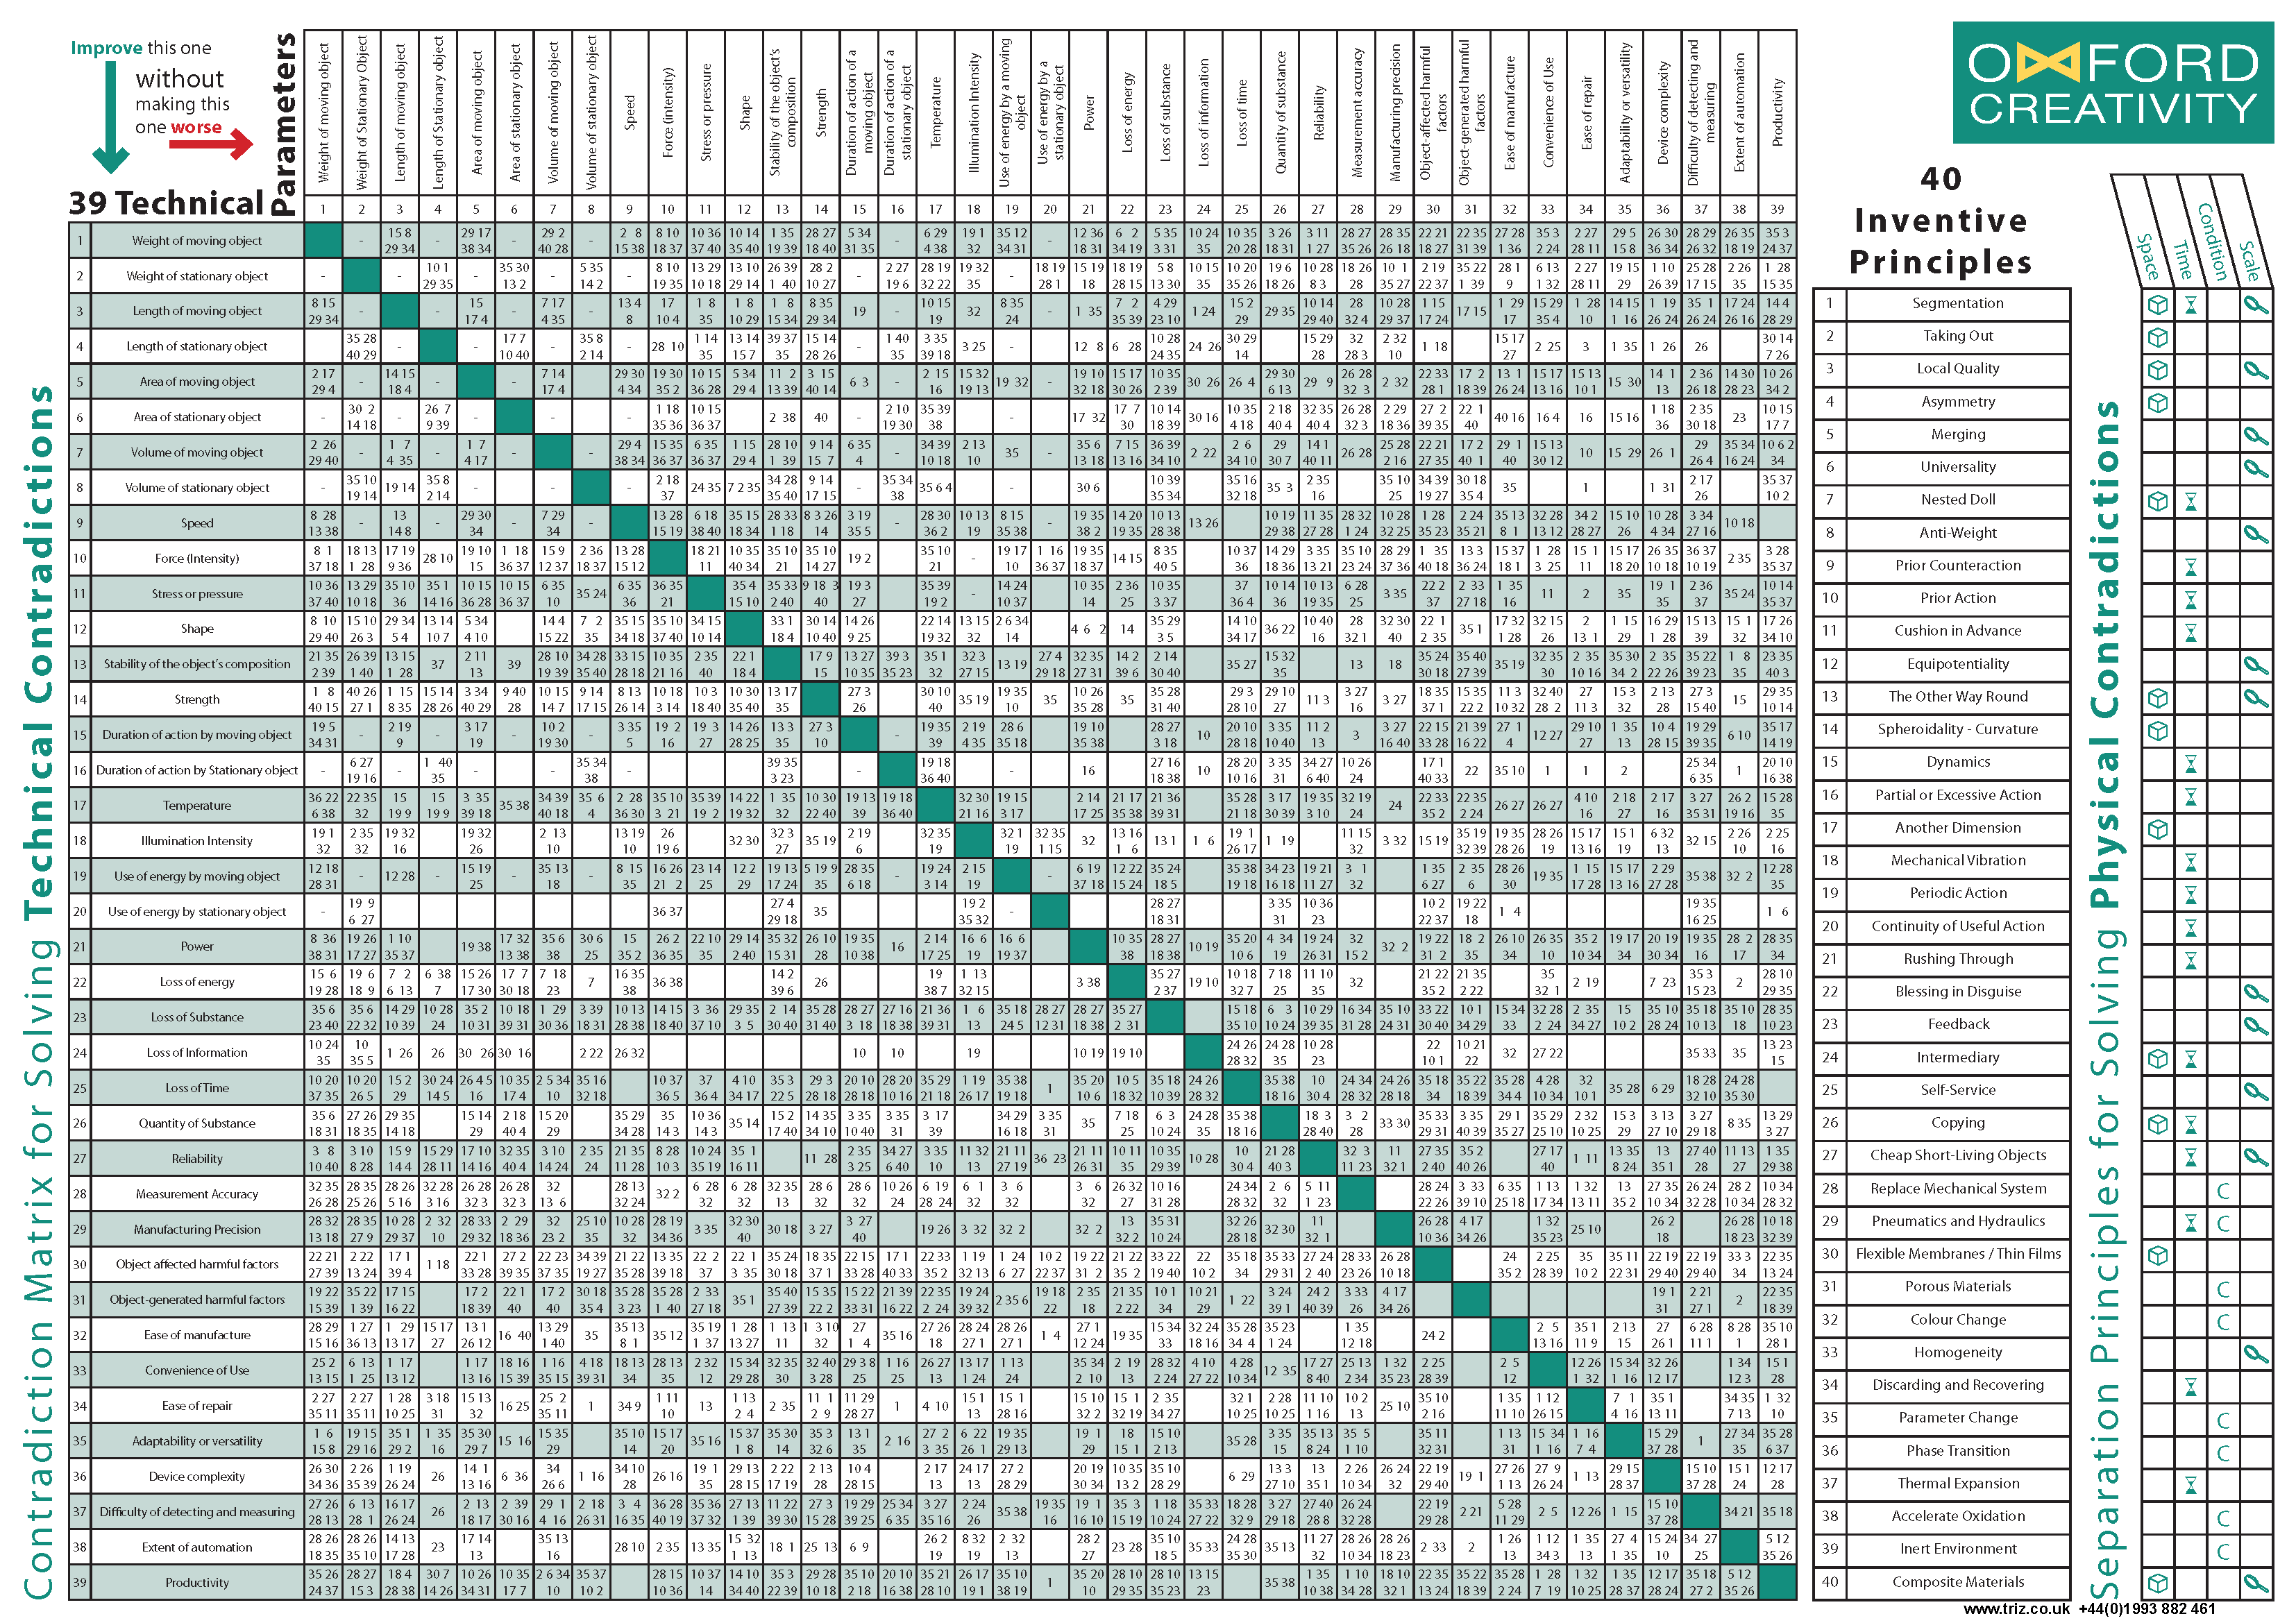
\includegraphics[width=\linewidth]{./images/triz_matrix.png}
						\caption{Example of a TRIZ Contradiction Matrix}
					\end{minipage}
					\hfill
					\begin{minipage}{0.35\linewidth}
						\centering
						
\includegraphics[width=0.8\linewidth]{./images/triz_qrcode.png}
						\caption{TRIZ 40 Principles}
					\end{minipage}
				\end{figure}

			\end{block}
			\vspace{1cm}

			\begin{block}{Strengths of TRIZ}
				\begin{itemize}
					\item Leverages past knowledge and proven inventive patterns
					\item Provides systematic tools for problem analysis and idea generation
					\item Helps resolve technical contradictions and optimize systems
					\item Widely applicable to various engineering and business domains
				\end{itemize}
			\end{block}


		\end{column}

		% Column 3
		\begin{column}{.3\linewidth}

			\begin{block}{Application to Social Challenges}
				Climate change is an urgent social challenge. Using TRIZ principles:
				\begin{itemize}
					\item \textbf{Preliminary Action (Principle 10):} Develop renewable energy and carbon capture ahead of crisis
					\item \textbf{Equipotentiality (Principle 12):} Balance carbon emissions and sequestration to reach net-zero
					\item \textbf{Partial or Excessive Actions (Principle 16):} Implement flexible carbon taxes and cap-and-trade schemes
					\item \textbf{Parameter Changes (Principle 35):} Transition to low-carbon economies and lifestyles
					\item \textbf{Composite Materials (Principle 40):} Deploy carbon fiber and green concrete for construction
				\end{itemize}
				\vspace{1.23cm}
				\begin{figure}
					\begin{tikzpicture}
						\begin{axis}[
								width=0.9\linewidth,
								height=0.5\linewidth,
								xlabel={Year},
								ylabel={Gigatons of CO2},
								ymin=0,
								legend pos=north east,
								tick label style={font=\tiny},
								legend style={font=\small},
								ymajorgrids=true,
								grid style=dashed,
								xticklabel style={/pgf/number format/1000 sep=},
							]
							\addplot coordinates {
									(2020, 36)
									(2025, 34)
									(2030, 31)
									(2035, 27)
									(2040, 22)
									(2045, 16)
									(2050, 10)
								};
							\addplot coordinates {
									(2020, 5)
									(2025, 7)
									(2030, 10)
									(2035, 14)
									(2040, 19)
									(2045, 25)
									(2050, 32)
								};
							\legend{Emissions, Carbon Removal}
						\end{axis}
					\end{tikzpicture}
					\caption{Projected Emissions and Carbon Removal Using TRIZ-based Solutions}
				\end{figure}
			\end{block}
			\vspace{1cm}
			\begin{block}{Impact of Innovation Methods}
				\begin{itemize}
					\item Design Thinking has been widely adopted by firms like Apple, Pepsi, and SAP to drive user-focused innovations
					\item TRIZ has helped companies like Intel, Samsung, and P\&G solve complex technical challenges and generate profitable patents
					\item Systematic innovation methods can amplify human creativity and accelerate progress on global economic and social challenges
				\end{itemize}
			\end{block}
			\vspace{1cm}
			\begin{block}{Conclusion}
				To make a positive impact as future leaders, we could:
				\begin{enumerate}
					\item Master systematic innovation methods like Design Thinking and TRIZ
					\item Apply these methods to analyze and solve complex real-world problems
					\item Combine empathy, creativity, and structured problem-solving approaches
					\item Generate innovative, human-centric solutions to economic and social challenges
				\end{enumerate}
			\end{block}

		\end{column}
	\end{columns}

\end{frame}
\end{document}